\chapter{Protocols and Security}

\section{Transport Choices}
TCP provides reliability; QUIC offers lower latency and built-in encryption. Smart Relay prefers QUIC where available and falls back to TCP for compatibility.

\section{TLS and Certificates}
Mutual TLS protects both client and server. Certificate automation (ACME) should be paired with automated renewal hooks that reload proxy cores without downtime.

\section{Tunneling Primer}
\begin{figure}[h]
    \centering
    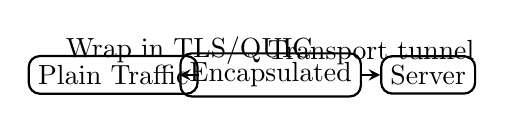
\begin{tikzpicture}[node distance=2cm,>=stealth,thick]
        \node (plain) [draw, rounded corners] {Plain Traffic};
        \node (encap) [draw, rounded corners, right of=plain] {Encapsulated};
        \node (server) [draw, rounded corners, right of=encap] {Server};
        \draw[->] (plain) -- node[above]{Wrap in TLS/QUIC} (encap);
        \draw[->] (encap) -- node[above]{Transport tunnel} (server);
    \end{tikzpicture}
    \caption{Encapsulation hides metadata and resists filtering.}
\end{figure}

\section{Threat Model Essentials}
\begin{itemize}
    \item Protect metadata (SNI, timing) using ESNI/QUIC and padding.
    \item Rotate endpoints and apply congestion-aware routing to avoid fingerprinting.
    \item Collect only minimal telemetry; strip IPs before storing.
\end{itemize}

\section{DNS and Blocking Evasion}
\begin{itemize}
    \item Prefer DoH/DoQ to hide DNS from on-path observers.
    \item Use domain fronting sparingly; validate terms of service of CDNs.
    \item Maintain fallback IP lists for cold-start when DNS is interfered.
\end{itemize}

